\documentclass[logo]{pbml}

\usepackage{clrscode}

\begin{document}


\title{Integrating Output from Specialized Modules in Machine Translation}

\subtitle{Transliterations in Joshua}


\author{firstname=Ann, surname=Irvine,
       address={Center for Language and Speech Processing, Johns Hopkins University}}
\author{firstname=Mike, surname=Kayser, address={BBN Technologies}}
\author{firstname=Zhifei, surname=Li,
        address={Center for Language and Speech Processing, Johns Hopkins University}}
\author{firstname=Wren, surname=Thornton,
        address={Cognitive Science Program, Indiana University}}
\author{firstname=Chris, surname=Callison-Burch,
        address={Center for Language and Speech Processing, Johns Hopkins University}}


%\shorttitle{Integrating Output from Specialized Modules in Machine Translation}
\shorttitle{Specialized Modules in MT}
%\shortauthor{A. Irvine, M. Kayser, Z. Li, W. Thornton, C. Callison-Burch}
\shortauthor{Irvine, Kayser, Li, Thornton, Callison-Burch}

\maketitle


\begin{abstract}
In many cases in SMT we want to allow specialized modules to propose translation fragments to the decoder and allow them to compete with translations contained in the phrase table. Transliteration is one module that may produce such specialized output. In this paper, as an example, we build a specialized Urdu transliteration module and integrate its output into an Urdu--English MT system. The module marks-up the test text using an XML format, and the decoder allows alternate translations (transliterations) to compete.
\end{abstract}

\section{Introduction}
The phrase tables used in statistical machine translation (SMT) systems are often incomplete, and they may not take full advantage of the linguistic knowledge that we have about a language. However, many data-driven NLP tools exist for specific linguistic tasks. For this reason, it is often useful to create specialized modules that employ other methods of translation not so dependent on the training text. Such modules may include noun phrase taggers and translators \cite{Koehn2004a}, morphological analyzers, modality taggers and translators,\footnote{Verbal modality expresses the notions of possibility, necessity, permission, and obligation} and transliteration systems. These modules may then be integrated into the MT pipeline \cite{Dugast2007, Yang2006}.

Previous SMT systems have integrated the subtask output of specialized modules using an XML-markup on input text \cite{Koehn2004b, Senellart2003}. Here we present an XML format to integrate the output of our specialized transliteration module into the Joshua decoder \cite{JoshuaWMT}. It necessarily differs from the XML schemes used in phrase-based decoders because Joshua is a parsing-based decoder. We illustrate its use with an example transliteration module.

\section{Decoding Constraints}
Joshua \cite{JoshuaWMT} is an open source\footnote{http://cs.jhu.edu/$\sim$ccb/joshua/} SMT system that uses synchronous context free grammars (SCFGs) as its underlying formalism. SCFGs provide a convenient and theoretically grounded way of incorporating linguistic information into statistical models of translation. Joshua implements all the essential algorithms described in \cite{Chiang2007} and supports Hiero-style rules \cite{Chiang2005} as well as richer syntax augmented rules \cite{Zollman2008}. The version of Joshua that we have used in this work incorporates the grammar extraction software that comes as part of their open source SAMT toolkit.\footnote{http://www.cs.cmu.edu/zollmann/samt/} Joshua translates by applying the extracted SCFG rules to the source language text using a general chart parsing framework \cite{PBML09}.

A probabilistic SCFG consists of a set of source-language terminal symbols $T_S$, a set of target-language terminal symbols $T_T$, a set of nonterminals $N$ that is shared between both languages, and set of production rules of the form
$$X \to \langle \gamma,\alpha,\sim,w \rangle$$
where $X \in N, \gamma \in [N \cup T_S]*$ is a (possibly mixed) sequence of nonterminals and source terminals that form the lefthand side of the rule, $\alpha \in [N \cup T_T]*$ is a  (again possibly mixed) sequence of nonterminals and target-language terminals that form the righthand side of the rule, and $\sim$ is a one-to-one correspondence between the nonterminals of $\gamma$ and $\alpha$. $w$ is a weight for the production rule.

To support integrating specialized modules we introduced the ability to specify alternate translation rules in the document to be translated. In order to support both the use of alternate translation rules and regular decoding (without alternate rules), we introduced a new parameter in Joshua's configuration file for specifying which parser to use on the input file. Each input file parser reads in the file and emits a sequence of segments to be translated. In order to avoid storing the whole file in memory, the sequence is returned as a co-iterator.\footnote{We use some object instance which implements the \texttt{joshua.util.CoIterator} interface. Both iterators and co-iterators are examples of abstractions over enumerations. Whereas an iterator captures the notion of producing the elements, a co-iterator captures the notion of consuming those elements.} By using a co-iterator, the sequence is produced lazily and consumed on-line, invoking the chart parser as a co-routine. To avoid interrupting translation in the middle of a file, we want to detect malformed files before translation begins. So in order to detect malformed file errors eagerly, the file is read once with a co-iterator that consumes the segments but does nothing with them, and then re-read to produce segments for the chart parser.

Each translation segment consists of an ID, a source sentence, and a collection of spans covering the sentence where each span contains a collection of constraints. Spans containing only soft constraints are allowed to overlap, whereas hard constraint spans may not overlap. Constraints are drawn from three types: lefthand side (LHS) constraints, righthand side (RHS) constraints, and rule constraints. LHS constraints are hard constraints specifying that the span be treated as a specified nonterminal, thus filtering the regular grammar to generate translations only from that nonterminal. One use for LHS constraints is to integrate chunking or tagging information before decoding. RHS constraints are hard constraints filtering the regular grammar such that only rules generating the desired translation can be used. A use for RHS constraints would be integrating word sense disambiguation before decoding. Rule constraints specify a new grammar rule including a LHS nonterminal, source RHS (derived from the source sentence), target RHS, and feature values. Rule constraints can be either hard or soft; if they are hard, they override the regular grammar; if they are soft, they are considered an addition to the regular grammar and will compete with regular rules. Rule constraints for any given span must be marked collectively as all hard or all soft.

\subsection{XML Markup}
The XML format follows straightforwardly from the specification of segments. The XML file must be valid XML, and thus must have a root element. Underneath the root element are some number of \texttt{<seg>} tags with a required \texttt{id} attribute that specifies the input segment number. The source sentence is given as raw text under the \texttt{<seg>} tag. Each \texttt{<seg>} tag may contain one or more \texttt{<span>} tags with required \texttt{start} and \texttt{end} attributes and an optional \texttt{hard} attribute for rule constraints. Each \texttt{<span>} tag must contain one or more \texttt{<constraint>} tags each of which contains an optional \texttt{<lhs>} tag, containing nonterminal text, followed by an optional \texttt{<rhs>} tag with an optional \texttt{features} attribute and containing target text. Any other tags are ignored by the XML parser.

This specification of the XML format is overly liberal and could admit files which are non-sensical or which cannot be represented internally. In order to rule out such files, the generated objects are run through a type checker to ensure semantic validity. The type checker verifies the following invariants:

\begin{itemize}
\item Each constraint adheres to one of the three types, thus it has
	\begin{itemize}
	\item only a \texttt{<lhs>} tag, or
	\item only a \texttt{<rhs>} tag with no \texttt{features} attribute, or
	\item a \texttt{<lhs>} tag, a \texttt{<rhs>}, and a \texttt{features} attribute
	\end{itemize}
\item For each span,
	\begin{itemize}
	\item the start and end indices are within the width of the sentence
	\item the start index is smaller than the end index
	\end{itemize}
\item There are no overlapping hard spans
\end{itemize}

While the \texttt{features} attribute is considered optional in terms of the DTD for the XML grammar, that is only because DTDs are unable to capture the dependency relation between the three valid constraint types.\footnote{XML Schema and RelaxNG are also unable to capture all the necessary dependency relations. Even if they can capture the tag and attribute dependencies between the three constraint types, type checking would still be necessary due to the context-sensitive restrictions on valid start and end indices depending on the length in words of the source text.} If both \texttt{<lhs>} and \texttt{<rhs>} tags are provided but there is no \texttt{feature} attribute, this is considered a type error since the constraint does not belong to any of the three types: LHS constraints do not have \texttt{<rhs>} tags, RHS constraints do not have \texttt{<lhs>} tags, and rule constraints require a \texttt{features} attribute.

\section{Decoder Integration}

To enforce the three kinds of constraints (i.e., rule, LHS, and RHS) during decoding, we modified the regular chart-based decoding algorithm in Joshua.
Rule constraints can be hard or soft.
A rule constraint provides a new translation option for a source span,
in addition to those translation options (hereafter called grammar-based translations) provided by the regular grammars.
If the rule constraint is hard, all the grammar-based translations
will be disallowed in the final translation output. Otherwise, the new translation option will
compete with those grammar-based translations, in a probabilistic manner.
Different from a rule constraint, LHS and RHS constraints are always hard, meaning that
a grammar-based translation will be disallowed if its LHS or RHS does not match the LHS or RHS constraint.

Figure \ref{alg-constraint-decoding} presents the
modified algorithm, where lines \ref{line1}, \ref{line2}, and \ref{line3} are added to
the regular chart-parsing algorithm in order to support manual constraints.
As shown in line \ref{line1}, the algorithm first adds the rule constraints (regardless of being soft or hard) into the chart
so that the decoding algorithm will consider these rule translations as candidate translations.
To support the \textbf{hard} constraints, the algorithm will run through two filtering processes.
In line \ref{line2}, if a span is within the coverage of a \textbf{hard} rule constraint,
all the grammar-based rules applicable to this span will be disallowed.
Similarly, all the applicable grammar rules that do not match
any LHS or RHS constraints for the span will be filtered out, as shown in line \ref{line3}.


\begin{figure}[t]
\begin{center}
\begin{codebox}
\Procname{$\proc{\bf DecodingWithConstraints}(\id{grammars}, \id{ sentence}, \id{ constraints})$}
\li Add the \textrm{rule} constraints into the Chart \label{line1}
%\li regular chart seeding%
%\li $\For \id{w}  \kw{in }  [1,n]$
%\li \> $\For \id{i}  \kw{in }  [0,n-w]$
%\li \> $j = i + w$ \Comment each span [i,j]
\li For each \textrm{span} $[i,j]$ with increasing length (i.e., $j-i+1$)
\li \> Identify applicable grammar rules for the span
\li \> Filter the grammar rules based on \textbf{hard} \textrm{rule} constraints \label{line2}
\li \> Filter the grammar rules based on \textrm{LHS} and \textrm{RHS} constraints \label{line3}
\li \> Add the surviving grammar rules into the chart
\end{codebox}
\end{center}
\caption{Constraining Chart-based Decoding with Manual Constraints.}
\label{alg-constraint-decoding}
\vspace{-0.1in}
\end{figure}

\section{Transliteration Module}
Here we present a specialized transliteration module that uses Joshua's new XML markup. We developed an Urdu-English transliterator, which is useful because our LDC Urdu Language Pack bilingual parallel corpus \footnote{LDC catalog number LDC2009E12, "NIST Open MT08 Urdu Resources"} has only 88,108 sentence pairs with 1,586,065 English tokens and 1,664,409 Urdu tokens. In this data, we observed that 2\% of words in a development set were out-of-vocabulary (OOV) with respect to the training bitext. With the help of a human annotator, we found that approximately 33\% of these words were phonetically transliterable; for example, proper names or borrowed words. Introducing a module for generating transliterations and integrating that output into the output of an end-to-end MT system clearly has the potential to improve performance.

\subsection{Basic Framework} \label{transliteration-framework}
We treat transliteration as a \emph{monotone character translation} task, similar to the work of \cite{Knight1997}. We used the Joshua MT system to build an Urdu transliteration module using a semantically-informed framework, described below, and several sources of transliteration pairs for training.

At training time, given a list of Urdu--English name pairs, we first perform character-to-character alignment using the freely available Berkeley Word Aligner.\footnote{http://code.google.com/p/berkeleyaligner/} Next, we find character-sequence pairs which conform to the alignment graph for a word pair; these are analogous to phrase pairs in phrase-based statistical MT. We build a table of such character-sequence mappings, annotated with translation probabilities. Finally we extract a frequency-annotated list of 1.3 million names from the English Gigaword corpus using a named entity tagger \cite{Finkel2009}. We then use this to train a character language model prior. Having trained these components, we use them in conjunction with the off-the-shelf Joshua MT decoder.

During decoding, a novel Urdu word is segmented into sequences of characters, and each character sequence is translated to an English character sequence. Unlike in the closely analogous process of phrasal machine translation, in phonetic transliteration the translated character sequences are never reordered. Transliteration hypotheses are scored using a log-linear model which makes use of character sequence translation scores and a character-LM prior score. The result is a single English phonetic gloss of the Urdu word.

\subsection{Semantically-targeted transliteration} \label{semantically-targeted-transliteration}
We trained two transliteration systems, one for person names and one for all other semantic types (including non-names). These two systems shared all components except for the character LM and the dataset used for decoder weight tuning. For the person-name transliteration system, we trained our character language model from the large list of English person names automatically extracted from the Gigaword corpus. In the non-person-name transliteration system, we trained a model from a large list of English words, without regard to semantic type.
	
\subsection{Training the module}
In order to train the transliteration module, we gathered pairs of names that were likely to be transliterations of one another. We obtained unique name pairs from three sources: the Urdu--English parallel corpus (about 2,000 pairs, extracted from alignments and checked by a human annotator), Amazon's Mechanical Turk system (over 12,000 pairs), and linked people pages from the Urdu and English Wikipedias (about 1,000 pairs). Our final system used about 15,000 pairs of Urdu--English transliterated name pairs.\footnote{The complete name pair list is freely available at http://www.clsp.jhu.edu/$\sim$anni/} Transliteration performance improved with increasing amounts of training data, and our final module outperformed the baseline system available from the LDC Urdu Language Pack.

\subsection{Integrating the module}
When using the rule constraint mechanism to add externally constructed theories to Joshua's search space, it is necessary to specify a left-hand-side nonterminal for each rule. Since this nonterminal label is used by Joshua in decoding, it is helpful to choose a label which accurately represents the grammatical content of the covered phrase. Rather than compute a single guess for this label, we add multiple arcs to the search space, each with a different nonterminal. We use the automatically determined named-entity-category of the source word to construct the set of possible labels for a transliterated word.

In particular, before decoding we compute from training the N most frequent target nonterminal labels assigned to low-frequency words of each source name category (the name categories are: Person, Location, Organization, Geopolitical Entity, Facility). At decoding time, we use an automatic name tagger to compute the semantic category of each source word. For every transliteration candidate, we add N arcs to the search space, each with a different label from the semantically-targeted set. In our experiments, we use the value N=5.

An example of the XML markup for an input Urdu sentence is shown in Figure \ref{example-urdu-xml}. In this example, two word spans are tagged with constraints and hypothesis transliterations. Each span and transliteration hypothesis is tagged with the N most frequent target nonterminal labels (e.g. NNP, NN, etc. for a PERSON tag).

\begin{figure}[t]
\begin{center}
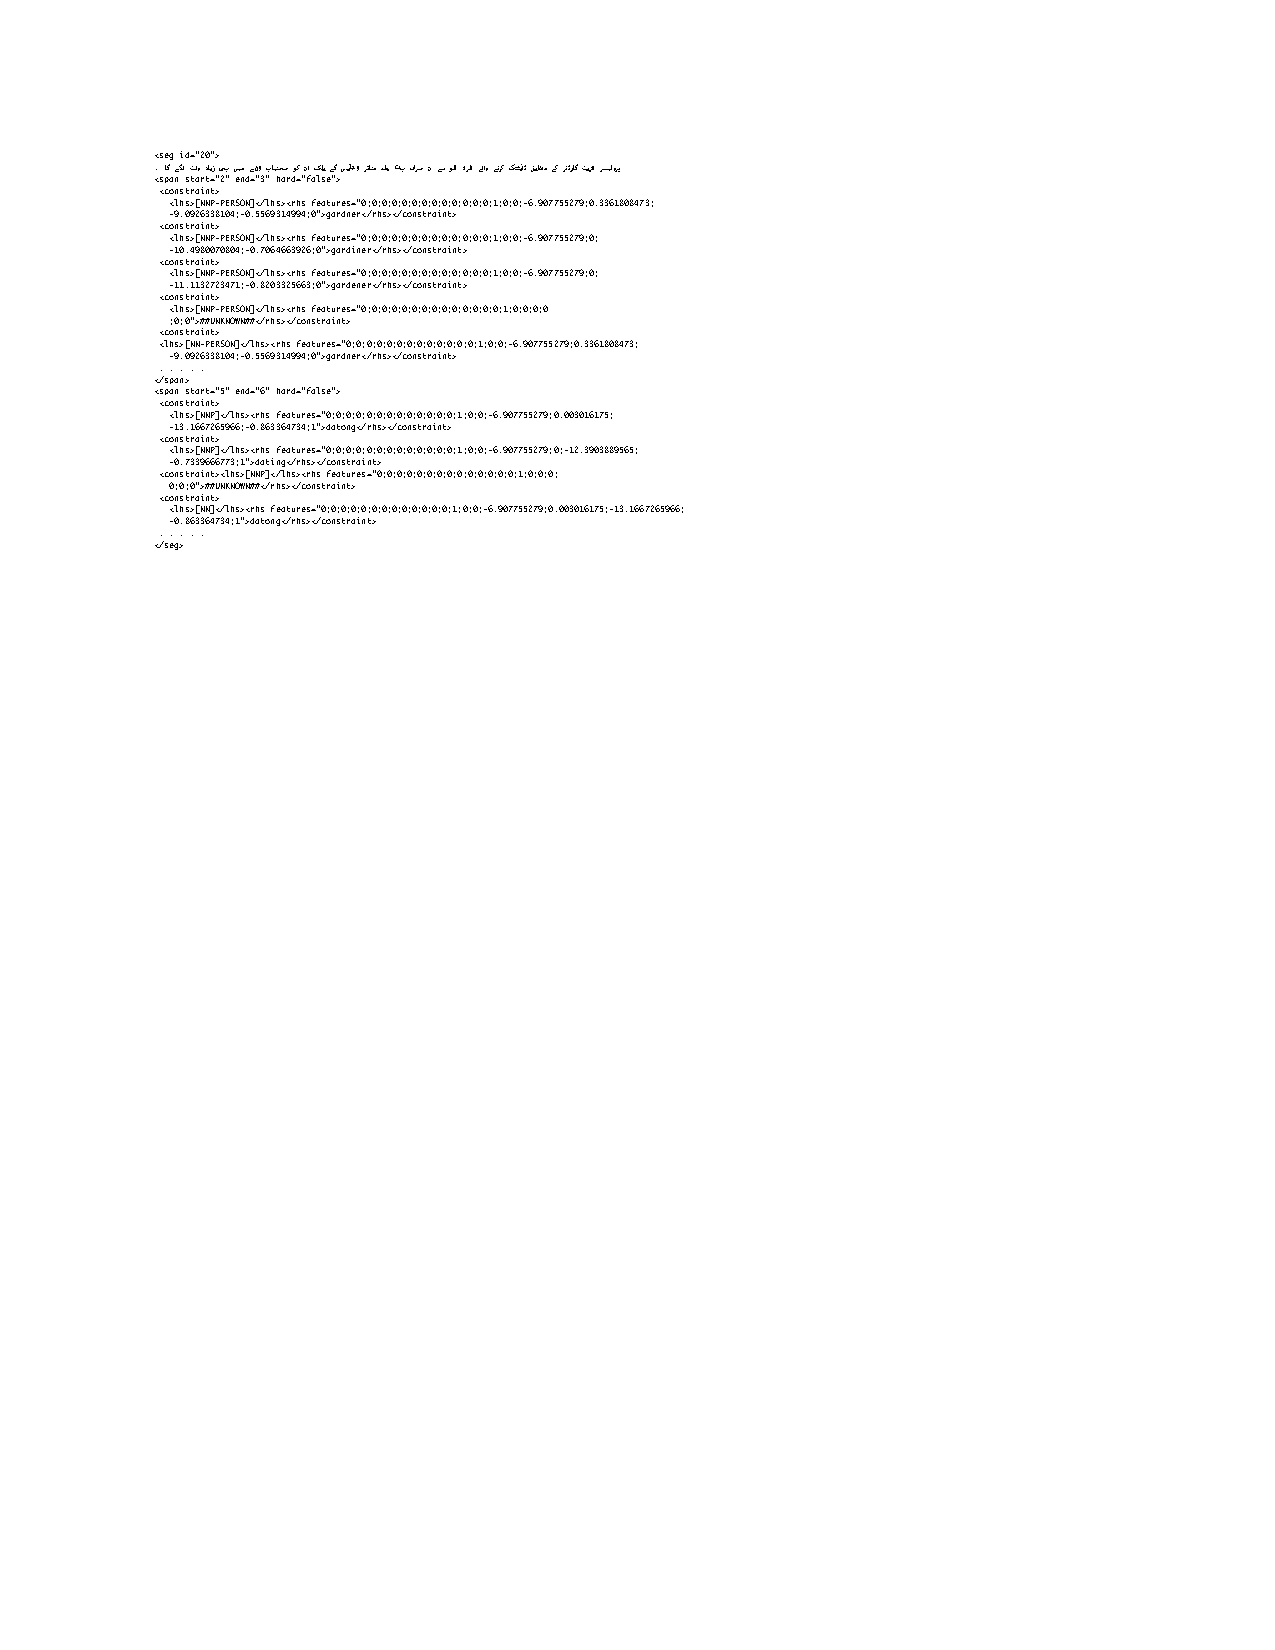
\includegraphics[height=3.5 in]{SampleSentence.pdf}
\end{center}
\caption{An example of XML markup on Urdu text.
Each span has 21 associated feature weights. The first 13 features represent the feature space of traditionally extracted Joshua translation rules. Since transliteration rules do not exist in the same feature space, these feature values are always set to 0 for transliteration rules.}
\label{example-urdu-xml}
\end{figure}

\section{Results}
We tested the impact of transliterator integration in a small number of blind submissions to the NIST MT09 Urdu--English evaluation. We integrated the transliterator into the current Joshua system. In one experiment, we transliterated all low-frequency words, while in a second experiment we transliterated only low-frequency person names. Our baseline for comparison was the identical Joshua system without transliterations.

We compared the baseline against the transliteration-aware systems both quantitatively and qualitatively. In a quantitative comparison, whose results are in Table \ref{transliteration-impact-quantitative}, transliteration yielded a small but notable BLEU improvement. As shown in the table, transliterating words of all semantic types yielded slightly better performance than transliterating only words marked as person names.

\begin{table}
\begin{center}
\begin{tabular}{|c|c|}
\hline
\textbf{Joshua Translation System} & \textbf{NIST MT09 BLEU Score} \\ \hline
No Transliteration & .2958 \\ \hline
Transliterate names only & .2980 \\ \hline
Transliterate all types & .3010 \\ \hline
\end{tabular}
\end{center}
\caption{\label{transliteration-impact-quantitative} Impact of transliteration on BLEU in submissions to NIST MT09 evaluation. }
\end{table}


We also qualitatively compared the best transliteration-aware system with the baseline system via manual inspection of decoder output. As expected, some sentences showed clear improvement via the increased lexical coverage allowed by the transliteration model, while other sentences showed little benefit. In some sentences, the transliteration model hypothesized incorrect transliterations for OOV words. More effectively filtering such incorrect translation options, such as through a more developed measure of confidence,  is a potential avenue for future work. Tables \ref{transliteration-impact-example1} and \ref{transliteration-impact-example2} show examples of Joshua decoder output with and without the transliteration feature.

\begin{table}
\begin{center}
\begin{tabular}{|c|p{8cm}|}
\hline
\small \textbf{Without Transliteration} & \small \textbf{[UNKNOWN]} Members said that the economic plan, expensive, and will not be effective. \\ \hline
\small \textbf{With Transliteration} & \small \textbf{Republican} members said that the economic plan, expensive, and will not be effective.  \\ \hline
\small \textbf{Reference} & \small The republican members said that this economic plan is very ``expensive'' and will not be effective. \\ \hline
\small \textbf{Without Transliteration} & However, \small \textbf{[UNKNOWN]} said that he \small \textbf{[UNKNOWN]} president to respect their age and are also due to yell at them, but they were saying truth from miles away.  \\ \hline
\small \textbf{With Transliteration} & ``However, \small \textbf{Erdogan} said that he respects the \small \textbf{Israeli} President and his age as a result of which they yell at them , but they were saying the truth from miles away.  \\ \hline
\small \textbf{Reference} & However, later \small \textbf{Erdogan} said that he respects \small \textbf{Israeli} President and his age as well which is why he did not yell at him but whatever he was saying was miles away from truth.   \\ \hline
\end{tabular}
\end{center}
\normalsize
\caption{\label{transliteration-impact-example1} Examples of improvements from transliteration.}
\end{table}


\begin{table}
\begin{center}
\begin{tabular}{|c|p{8cm}|}
\hline
\small \textbf{Without Transliteration} & In southern germany \small \textbf{[UNKNOWN]} a resident of the area of \small \textbf{[UNKNOWN]} \small \textbf{[UNKNOWN]} has left behind a big business group  \\ \hline
\small \textbf{With Transliteration} & A resident of the area of \small \textbf{Cuba} in south Germany \small \textbf{Adolf Merkel} has left behind a big business group  \\ \hline
\small \textbf{Reference} & \small \textbf{Adolf Merckle} of southern Germany's \small \textbf{Swabia} area has left a large business group behind  \\ \hline
\end{tabular}
\end{center}
\normalsize
\caption{\label{transliteration-impact-example2} Impact of transliteration. Note that the location name ``Swabia'' was incorrectly transliterated to ``Cuba.'' This example indicates the future room for improvement.}
\end{table}

\section{Conclusion}
\vspace{-.15cm}
In this work, we created an XML format to markup the output of specialized subtask modules and integrate alternate translations into the SMT decoder. We created a transliteration module using a character-based statistical MT system and several thousand pairs of transliterated words.  The results are promising. In particular, a qualitative analysis suggests that the transliterations were able to appropriately compete with the phrase-based translation output. This work has also opened the door to integrating additional specialized translation modules. Such modules have a potential to increase translation performance, particularly in low-resource conditions.\footnote{This research was supported in part by the European Commission through the EuroMatrixPlus project, by the US National Science Foundation under grant IIS-0713448, and by the Human Language Technology Center of Excellence.  Any opinions, findings, and conclusions or recommendations expressed in this material are the authors' and do not necessarily reflect the views of the sponsor. }


\bibliography{mt_mar_translit}

\end{document}
